\section{Sets, Functions and Graphs}

\begin{answer}
  Important notations:
  \begin{itemize}
    \item Curly brackets (i.e. $\left\{  \right\}$) represent a set.
    \item The empty set is written as $\varnothing$.
    \item $x\in A$ means $x$ is an element of the set $A$, and $y\notin A$ means that $y$ is not an element of $A$.
    \item $\wedge$ and $\vee$ mean \textit{and} and \textit{or}, respectively. 
    \item Natural numbers: $\mathbb{N}=\left\{ 1,2,3,\dots \right\}$.\\(By some definitions $0\in\mathbb{N}$, by others $0\notin\mathbb{N}$)
    \item Integers: $\mathbb{Z}=\left\{ 0,\pm 1,\pm 2,\dots \right\}$.
    \item Rational numbers: $\mathbb{Q}=\left\{ \frac{p}{q} \mid p,q\in\mathbb{Z}, q\neq0\right\}$.
    \item Real numbers: $\mathbb{R}=\left\{ x \mid x\in\left( -\infty,\infty \right) \right\}$.\\(The formal definition is too complicated for this course\footnote{Some formal definitions can be found here: \url{https://en.wikipedia.org/wiki/Construction_of_the_real_numbers}.})
    \item Complex numbers: $\mathbb{C}=\left\{ x+iy \mid x,y\in\mathbb{R},\ i^{2}=-1 \right\}$.
  \end{itemize}
\end{answer}

\subsection{Sets}
\begin{enumerate}
  \item Write the following sets explicitly:

    \begin{enumerate}
      \item $A=\left\{ x\in \mathbb{N}\mid1<x\leq7\right\}$
        \if\withsol1{
            \begin{answer}
              While $1$ is not included in the set (since $1<x$), the number $7$ is, since $x\leq7$.

              Hence: $A=\left\{ 2,3,4,5,6,7 \right\}$.
          \end{answer}}
        \fi

      \item $A=\left\{ x\in \mathbb{Z}\mid x<5\right\}$
        \if\withsol1{

            \begin{answer}
              $\mathbb{Z}$ is the set of all integers, including $0$. Therefore: $A=\left\{ \dots,-2,-1,0,1,2,3,4 \right\}$.
          \end{answer}}
        \fi
      \item $A=\left\{ x\in \mathbb{R}\mid x^{2}=-1 \right\}$
        \if\withsol1{

            \begin{answer}
              The solution for $x^{2}=-1$ is not a real number, and therefore $A=\varnothing$.
          \end{answer}}
        \fi

      \item $A=\left\{ x\in \mathbb{N} \wedge x\in \mathbb{Q} \right\}$
        \if\withsol1{

            \begin{answer}
              All integers are also rational, and therefore $A=\mathbb{N}$.
          \end{answer}}
        \fi
      \item $A=\left\{ x\in \mathbb{R} \mid x^{2}-3x-4=0 \right\}$
        \if\withsol1{

            \begin{answer}
              Using the quadratic equation solution $\left(ax^{2}+bx+c=0 \Rightarrow x_{1,2}=\frac{-b\pm\sqrt{b^{2}-4ac}}{2a}\right)$ yields $x_{1,2}=-1,4$.

              This means $A=\left\{ -1, 4 \right\}$.
          \end{answer}}
        \fi
      \item $A=\left\{ x\in\mathbb{R}\mid x<5\wedge x \geq 2\right\}$
        \if\withsol1{

            \begin{answer}
              $x=\left[2,5\right)$
          \end{answer}}
        \fi
    \end{enumerate}

  \item Determine the relation between the sets:
    \begin{enumerate}
      \item $\mathbb{R},\ \mathbb{Q},\ \mathbb{Z},\ \mathbb{N}$
        \if\withsol1{

            \begin{answer}
              $\mathbb{R}\supset\mathbb{Q}\supset\mathbb{Z}\supset\mathbb{N}$
          \end{answer}}
        \fi

      \item $A=\left\{ 1,\ 2,\ 3\right\},\ B=\left\{ 1,\ 2 \right\}$
        \if\withsol1{

            \begin{answer}    
              $A\supset B$
          \end{answer}}
        \fi


      \item $A=\varnothing,\ B=\left\{ 2,\ -5,\ \pi \right\}$
        \if\withsol1{

            \begin{answer}
              $A\subset B$
          \end{answer}}
        \fi

      \item $A=\mathbb{Z},\ B=\left\{ \pm x \mid x\in\mathbb{N} \cup \right\{0\left\} \right\}$
        \if\withsol1{

            \begin{answer}
              $A=B$
          \end{answer}}
        \fi
      \item $A=\left\{\pi, e, \sqrt(2)\right\},\ B=\mathbb{Q}$
        \if\withsol1{

            \begin{answer}
              All the numbers in $A$ are irrational and thus do not belong to $B$, meaning $A\cap B = \varnothing$.
          \end{answer}}
        \fi
    \end{enumerate}

    \if\withsol1{\newpage}\fi

  \item Using Venn diagrams, show the following relations:
    \def\firstcircle{(0,0) circle (1.5cm)}
    \def\secondcircle{(0:2cm) circle (1.5cm)}
    \def\thirdcircle{(45:2cm) circle (1.5cm)}
    \def\spacerect{(-2cm,-2cm) rectangle (4cm,2cm)}

    \begin{enumerate}
      \item $A\cup B=B\cup A$ \tikzmarknode{top1}{}
      \item $A\cap B=B\cap A$ \tikzmarknode{bottom1}{}
        \if\withsol1{
            \VerticalBrace[thick, blue!70]{top1}{bottom1}{\color{blue!70}Commutative laws}
            \\~\\
            \begin{answer}
              \begin{minipage}{0.45\textwidth}
                \centering
                \begin{tikzpicture}
                  \begin{scope}
                  \end{scope}
                  \draw[thick, fill=blue!30] \firstcircle;
                  \draw[thick, fill=blue!30] \secondcircle;
                  \draw \firstcircle  node [] {$A$};
                  \draw \secondcircle node [] {$B$};
                \end{tikzpicture}
                $A\cup B=B\cup A$
              \end{minipage}
              \begin{minipage}{0.45\textwidth}
                \centering
                \begin{tikzpicture}
                  \begin{scope}
                    \clip \firstcircle;
                    \draw[thick] \firstcircle;
                    \draw[thick, fill=red!30] \secondcircle;
                  \end{scope}
                  \draw \firstcircle  node [] {$A$};
                  \draw \secondcircle node [] {$B$};
                \end{tikzpicture}

                $A\cap B=B\cap A$
              \end{minipage}
            \end{answer}
          }\fi
        \item $\left(A\cup B\right)\cup C=A\cup \left(B\cup C\right)$ \tikzmarknode{top2}{}
        \item $\left(A\cap B\right)\cap C=A\cap \left(B\cap C\right)$ \tikzmarknode{bottom2}{}
          \if\withsol1{
              \VerticalBrace[thick, blue!70]{top2}{bottom2}{\color{blue!70}Associative laws}
              \\~\\
              \begin{answer}
                \begin{minipage}{0.45\textwidth}
                  \centering
                  \begin{tikzpicture}
                    \begin{scope}
                    \end{scope}
                    \draw[thick, fill=green!30] \firstcircle;
                    \draw[thick, fill=green!30] \secondcircle;
                    \draw[thick, fill=green!30] \thirdcircle;
                    \draw \firstcircle  node [below] {$A$};
                    \draw \secondcircle node [below] {$B$};
                    \draw \thirdcircle  node [above] {$C$};
                  \end{tikzpicture}

                  $\left(A\cup B\right)\cup C=A\cup \left(B\cup C\right)$
                \end{minipage}
                \begin{minipage}{0.45\textwidth}
                  \centering
                  \begin{tikzpicture}
                    \begin{scope}
                      \clip \firstcircle;
                      \clip \secondcircle;
                      \draw[thick] \firstcircle;
                      \draw[thick] \secondcircle;
                      \draw[thick, fill=orange!30] \thirdcircle;
                    \end{scope}
                    \draw \firstcircle  node [below] {$A$};
                    \draw \secondcircle node [below] {$B$};
                    \draw \thirdcircle  node [above] {$C$};
                  \end{tikzpicture}

                  $\left(A\cap B\right)\cap C=A\cap \left(B\cap C\right)$
                \end{minipage}
              \end{answer}
            }\fi
          \item $A\cup\left(B\cap C\right)=\left(A\cup B\right)\cap\left(A\cup C\right)$ \tikzmarknode{top3}{}
          \item $A\cap\left(B\cup C\right){}=\left(A\cap B\right)\cup\left(A\cap C\right)$ \tikzmarknode{bottom3}{}
            \if\withsol1{
                \VerticalBrace[thick, blue!70]{top3}{bottom3}{\color{blue!70}Distributive laws}
                \\~\\
                \begin{answer}
                  \begin{minipage}{0.45\textwidth}
                    \centering
                    \begin{tikzpicture}
                      \begin{scope}
                        \draw[thick, fill=blue!30] \firstcircle;
                        \clip \secondcircle;
                        \draw[thick] \secondcircle;
                        \draw[thick, fill=blue!30] \thirdcircle;
                      \end{scope}
                      \draw \firstcircle  node [below] {$A$};
                      \draw \secondcircle node [below] {$B$};
                      \draw \thirdcircle  node [above] {$C$};
                    \end{tikzpicture}

                    $A\cup\left(B\cap C\right)=\left(A\cup B\right)\cap\left(A\cup C\right)$
                  \end{minipage}
                  \begin{minipage}{0.45\textwidth}
                    \centering
                    \begin{tikzpicture}
                      \begin{scope}
                        \draw[thick, fill=white] \firstcircle;
                        \clip \secondcircle \thirdcircle;
                        \draw[thick, fill=green!30] \firstcircle;
                        \draw[thick] \secondcircle;
                        \draw[thick] \thirdcircle;
                      \end{scope}
                      \draw \firstcircle  node [below] {$A$};
                      \draw \secondcircle node [below] {$B$};
                      \draw \thirdcircle  node [above] {$C$};
                    \end{tikzpicture}

                    $A\cap\left(B\cup C\right)=\left(A\cap B\right)\cup\left(A\cap C\right)$  
                  \end{minipage}
                \end{answer}
              }\fi
            \item $\left(A\cup B\right)^{C}=A^{C}\cap B^{C}$ \tikzmarknode{top4}{}
            \item $\left(A\cap B\right)^{C}=A^{C}\cup B^{C}$ \tikzmarknode{bottom4}{}
              \if\withsol1{
                  \VerticalBrace[thick, blue!70]{top4}{bottom4}{\color{blue!70}De Morgan's laws}
                  \\~\\
                  \begin{answer}
                    \begin{minipage}{0.45\textwidth}
                      \centering
                      \begin{tikzpicture}
                        \begin{scope}
                        \end{scope}
                        \draw[thick, fill=red!30] \spacerect;
                        \draw[thick, fill=white]  \firstcircle;
                        \draw[thick, fill=white]  \secondcircle;
                        \draw \firstcircle  node [] {$A$};
                        \draw \secondcircle node [] {$B$};
                      \end{tikzpicture}

                      $\left(A\cup B\right)^{C}=A^{C}\cap B^{C}$
                    \end{minipage}
                    \begin{minipage}{0.45\textwidth}
                      \centering
                      \begin{tikzpicture}
                        \begin{scope}
                          \draw[thick, fill=blue!30] \spacerect;
                          \clip \firstcircle;
                          \clip \secondcircle;
                          \draw[thick, fill=white]  \firstcircle;
                          \draw[thick, fill=white]  \secondcircle;
                        \end{scope}
                        \draw \firstcircle  node [] {$A$};
                        \draw \secondcircle node [] {$B$};
                      \end{tikzpicture}

                      $\left(A\cap B\right)^{C}=A^{C}\cup B^{C}$
                    \end{minipage}
                  \end{answer}
                }\fi
            \end{enumerate}

          \item Cartesian products:
            \begin{enumerate}
              \item What is the Cartesian product of $A=\left\{ x,\ y,\ z \right\}$ and $B=\left\{ a,\ b,\ c \right\}$?
                \if\withsol1{

                    \begin{answer}   
                      $A\times B=\left\{
\begin{pycode}
A = ['x', 'y', 'z']
B = ['a', 'b', 'c']
prod = ['\\left({}, {}\\right)'.format(i, j)
        for i in A
        for j in B]
print(',\\ '.join(prod))
\end{pycode}
                      \right\}$
                  \end{answer}}
                \fi

              \item Is the following true: $\left( x,\ a \right)=\left( a,\ x \right)$?
                \if\withsol1{

                    \begin{answer}
                      Generally not, only if $x=a$.
                  \end{answer}}
                \fi

              \item What is $B^{2}$? What is $A^{3}?$
                \if\withsol1{

                    \begin{answer}
\begin{pycode}
A = ['x', 'y', 'z']
A3 = ['\\left({}, {}, {}\\right)'.format(i, j, k)
      for i in A
      for j in A
      for k in A]
p0 = ',\\ '.join(A3[:9])
p1 = ',\\ '.join(A3[9:18])
p2 = ',\\ '.join(A3[18:])

B = ['a', 'b', 'c']
B2 = ['\\left({}, {}\\right)'.format(i, j)
      for i in B
for j in B]

print('\\begin{align*}')
print('B^{{2}}&=\\{{ {} \\}}\\\\'.format(',\\ '.join(B2)))
print('A^{3}&=\{')
print(p0, ',\\\\&', p1, ',\\\\&', p2)
print('\}')
print('\\end{align*}')
\end{pycode}
                  \end{answer}}
                \fi
            \end{enumerate}

          \item Extra: Prove that $\sqrt{2}$ is irrational.
            (In formal writing: $\nexists p,q\in\mathbb{Z}\rightarrow \sqrt{2}=\frac{p}{q}$. Simply written: $\sqrt{2}\notin\mathbb{Q}$)
            \if\withsol1{

                \begin{itemize}
                  \item[]
                    \begin{answer}
                      \begin{proof}
                        Suppose $\sqrt{2}$ is rational. This means that there exist two integers $p,q$ so that
                        \begin{equation}
                          \label{eq:sqrt2eq}
                          \sqrt{2}=\frac{p}{q}
                        \end{equation}
                        We may assume that $p$ and $q$ have no common factors, otherwise we cancel them out.\\
                        Squaring both sides of equation (\ref{eq:sqrt2eq}) yields
                        \begin{equation}
                          \label{eq:square}
                          2=\frac{p^{2}}{q^{2}}
                        \end{equation}
                        which means
                        \begin{equation}
                          \label{eq:p_even}
                          p^{2}=2q^{2}
                        \end{equation}
                        i.e. $p^{2}$ is even. This is only possible if $p$ is even, which by itself means that $p^2$ is divisible by $4$.\\
                        But if $p^{2}$ is divisible by $4$ then $2q^{2}$ is divisible by $4$ (due to equation (\ref{eq:p_even})) and thus $q^{2}$ is divisible by $2$, which means $p$ and $q$ have a common factor (i.e. $2$), in contradiction to our assumption.\\
                        Therefore $\sqrt{2}\notin\mathbb{Q}$.
                      \end{proof}
                    \end{answer}
                \end{itemize}
              }
            \fi
        \end{enumerate}


        \subsection{Functions}
        \begin{enumerate}
          \item Which of the following figures represent functions? Which of these functions are injective, surjective and/or bijective?

            \begin{minipage}{0.45\textwidth}
              \centering
              \begin{tikzpicture}[
                  every node/.style={on grid},
                  setA/.style={fill=red!50!gray,circle,inner sep=2pt},
                  every fit/.style={draw,fill=red!20,ellipse,text width=25pt},
                  >=latex
                ]

  % set A
                \node[setA,label=left:$a$] (a) {};
                \node[setA,below = of a,label=left:$b$] (b) {};
                \node[setA,below = of b,label=left:$c$] (c) {};
                \node[above=of a,anchor=south] {$A$};

  % set B
                \node[inner sep=0pt,right=3cm of a] (alpha) {$\alpha$};
                \node[below = of alpha] (beta) {$\beta$};
                \node[inner sep=0pt,below = of beta] (gamma) {$\gamma$};
                \node[above=of alpha,anchor=south] {$B$};

  % the arrows
                \draw[->,shorten >= 3pt] (a) -- node[] {} (alpha);
                \draw[->,shorten >= 3pt] (b) -- node[] {} (alpha);
                \draw[->,shorten >= 3pt] (c) -- node[] {} (beta);

  % the boxes around the sets
                \begin{pgfonlayer}{background}
                  \node[fit= (a) (c)] {};
                  \node[fit= (alpha) (gamma)] {};
                \end{pgfonlayer}
              \end{tikzpicture}

              (1)
            \end{minipage}%
            \begin{minipage}{0.45\textwidth}
              \centering
              \begin{tikzpicture}[
                  every node/.style={on grid},
                  setA/.style={fill=green!50!gray,circle,inner sep=2pt},
                  every fit/.style={draw,fill=green!20,ellipse,text width=25pt},
                  >=latex
                ]

  % set A
                \node[setA,label=left:$a$] (a) {};
                \node[setA,below = of a,label=left:$b$] (b) {};
                \node[setA,below = of b,label=left:$c$] (c) {};
                \node[above=of a,anchor=south] {$A$};

  % set B
                \node[inner sep=0pt,right=3cm of a] (alpha) {$\alpha$};
                \node[below = of alpha] (beta) {$\beta$};
                \node[inner sep=0pt,below = of beta] (gamma) {$\gamma$};
                \node[above=of alpha,anchor=south] {$B$};

  % the arrows
                \draw[->,shorten >= 3pt] (a) -- node[] {} (alpha);
                \draw[->,shorten >= 3pt] (b) -- node[] {} (alpha);
                \draw[->,shorten >= 3pt] (c) -- node[] {} (beta);
                \draw[->,shorten >= 3pt] (c) -- node[] {} (gamma);

  % the boxes around the sets
                \begin{pgfonlayer}{background}
                  \node[fit= (a) (c)] {};
                  \node[fit= (alpha) (gamma)] {};
                \end{pgfonlayer}
              \end{tikzpicture}

              (2)
            \end{minipage}

            \begin{minipage}{0.45\textwidth}
              \centering
              \begin{tikzpicture}[
                  every node/.style={on grid},
                  setA/.style={fill=blue!50!gray,circle,inner sep=2pt},
                  every fit/.style={draw,fill=blue!20,ellipse,text width=25pt},
                  >=latex
                ]

  % set A
                \node[setA,label=left:$a$] (a) {};
                \node[setA,below = of a,label=left:$b$] (b) {};
                \node[setA,below = of b,label=left:$c$] (c) {};
                \node[setA,below = of c,label=left:$d$] (d) {};
                \node[above=of a,anchor=south] {$A$};

  % set B
                \node[inner sep=0pt,right=3cm of a] (alpha) {$\alpha$};
                \node[below = of alpha] (beta) {$\beta$};
                \node[inner sep=0pt,below = of beta] (gamma) {$\gamma$};
                \node[inner sep=0pt,below = of gamma] (delta) {$\delta$};
                \node[above=of alpha,anchor=south] {$B$};

  % the arrows
                \draw[->,shorten >= 3pt] (a) -- node[] {} (beta);
                \draw[->,shorten >= 3pt] (b) -- node[] {} (alpha);
                \draw[->,shorten >= 3pt] (c) -- node[] {} (gamma);
                \draw[->,shorten >= 3pt] (d) -- node[] {} (delta);

  % the boxes around the sets
                \begin{pgfonlayer}{background}
                  \node[fit= (a) (d)] {};
                  \node[fit= (alpha) (delta)] {};
                \end{pgfonlayer}
              \end{tikzpicture}

              (3)
            \end{minipage}
            \begin{minipage}{0.45\textwidth}
              \centering
              \begin{tikzpicture}[
                  every node/.style={on grid},
                  setA/.style={fill=orange!70,circle,inner sep=2pt},
                  every fit/.style={draw,fill=orange!20,ellipse,text width=25pt},
                  >=latex
                ]

  % set A
                \node[setA,label=left:$a$] (a) {};
                \node[setA,below = of a,label=left:$b$] (b) {};
                \node[setA,below = of b,label=left:$c$] (c) {};
                \node[setA,below = of c,label=left:$d$] (d) {};
                \node[above=of a,anchor=south] {$A$};

  % set B
                \node[inner sep=0pt,right=3cm of a] (alpha) {$\alpha$};
                \node[below = of alpha] (beta) {$\beta$};
                \node[inner sep=0pt,below = of beta] (gamma) {$\gamma$};
                \node[above=of alpha,anchor=south] {$B$};

  % the arrows
                \draw[->,shorten >= 3pt] (a) -- node[] {} (beta);
                \draw[->,shorten >= 3pt] (b) -- node[] {} (alpha);
                \draw[->,shorten >= 3pt] (c) -- node[] {} (gamma);
                \draw[->,shorten >= 3pt] (d) -- node[] {} (gamma);

  % the boxes around the sets
                \begin{pgfonlayer}{background}
                  \node[fit= (a) (d)] {};
                  \node[fit= (alpha) (gamma)] {};
                \end{pgfonlayer}
              \end{tikzpicture}

              (4)
            \end{minipage}
            \if\withsol1{

                \begin{answer}
                  \begin{itemize}
                    \item Functions: (1) (3) (4). Number (2) is not a function, since c has two corresponding values in B.
                    \item Injective: (3). Both functions (1) and (4) have two values in A that corresponding to the same value in B.
                    \item Surjective: (3) (4). Function (1) has a value in B, $\gamma$, that does not correspond to any value in A.
                    \item Bijective: (3).
                  \end{itemize}
              \end{answer}}
            \fi

          \item \label{item:functions}Which of the following functions are injective over $\mathbb{R}$?
            \begin{enumerate}
              \item $f\left( x \right)=x^{2}$
              \item $f\left( x \right)=x^{3}$
              \item $f\left( x \right)=\sin\left( x \right)$
              \item $f\left( x \right)=\log\left( x \right)$\\(in the context of this course, $\log\left( x \right)$ is the natural logarithm, also known as $\ln\left( x \right)$)
              \item $f\left( x \right)=\left|x\right|$
              \item $f\left( x \right)=\sqrt{x}$
            \end{enumerate}
            \if\withsol1{

                \begin{answer}
                  Functions (2) and (4) are injective.
                  Function (1) is not injective, for example: $f\left( -2 \right)=\left( -2 \right)^{2}=4=2^{2}=f\left( 2 \right)$.

                  Function (3) is also not injective, for example: $f\left( \pi \right)=\sin\left( \pi \right)=0=\sin\left( 2\pi \right)=f\left( 2\pi \right)$.

                  Function (5) is also not injective, for example: $\text{abs}\left( -2 \right) = \text{abs}\left( 2 \right) = 2$.

                  ~\\
                  See the following graphs, representing the functions 1-6:
                  \centering{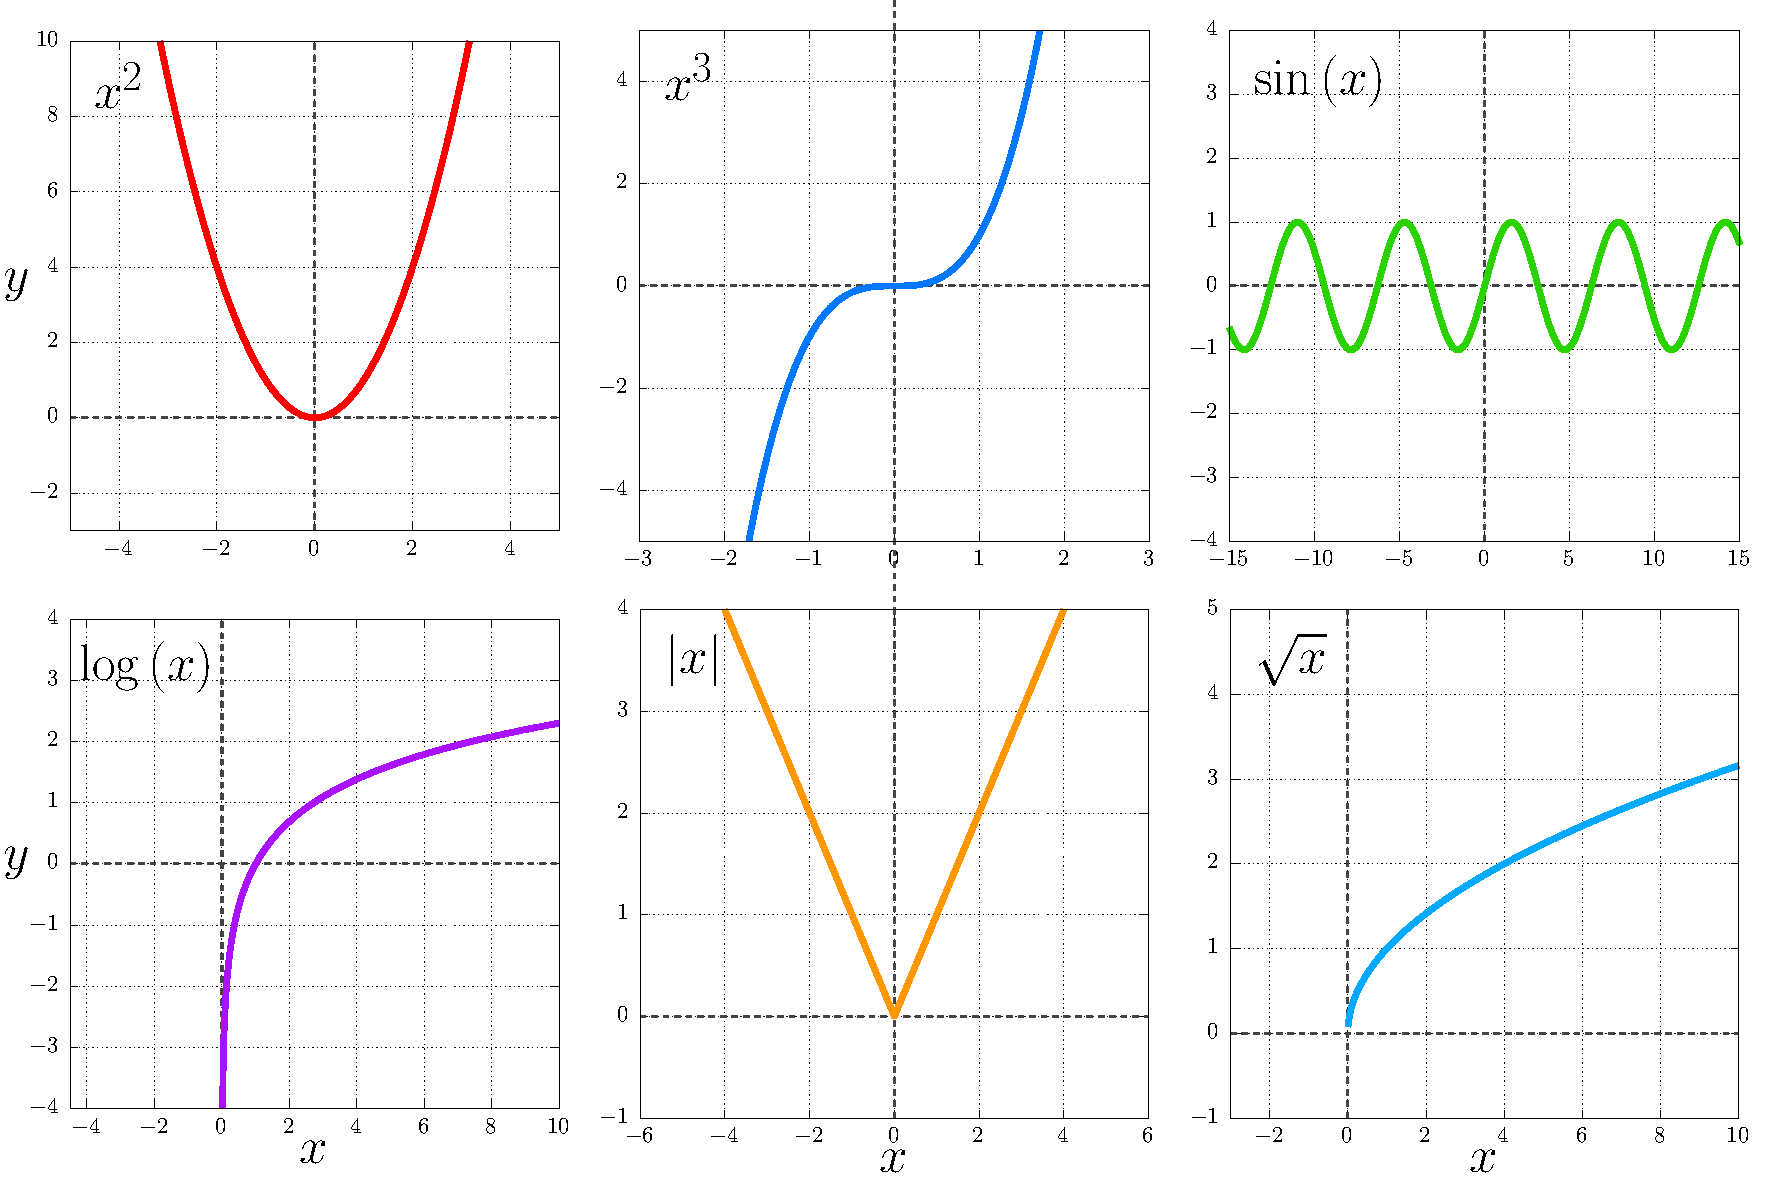
\includegraphics[scale=0.5]{figs/func_graphs.pdf}}
              \end{answer}}
            \fi

          \item Find the images of the functions from \ref{item:functions}.
            \if\withsol1{

                \begin{answer}
                  \begin{enumerate}
                    \item $\text{Im}\left(x^{2}\right)=\mathbb{R}_{0}^{+}=\mathbb{R}^{+}\cup\left\{ 0 \right\}=\left[0,\infty\right)$ (i.e. non-negative real numbers)
                    \item $\text{Im}\left(x^{3}\right)=\mathbb{R}$
                    \item $\text{Im}\left(\sin\left( x\right) \right)=\left[ -1,1 \right]$
                    \item $\text{Im}\left(\log\left( x\right) \right)=\mathbb{R}$
                    \item $\text{Im}\left(\left|x\right|\right)=\mathbb{R}_{0}^{+}$
                    \item $\text{Im}\left(\sqrt{x}\right)=\mathbb{R}_{0}^{+}$
                  \end{enumerate}
              \end{answer}}
            \fi

          \item For each of the injective functions from \ref{item:functions}, find its inverse.
            \if\withsol1{

                \begin{answer}
                  \begin{enumerate}
                    \item $f\left( x \right)=x^{3}\longrightarrow f^{-1}\left( y \right)=\sqrt[3]{y}$
                    \item $f\left( x \right)=\log\left( x \right)\longrightarrow f^{-1}\left( y \right)=e^{y}$
                    \item $f\left( x \right)=\sqrt{x}\longrightarrow f^{-1}\left( y \right)=y^{2}$
                  \end{enumerate}
              \end{answer}}
            \fi

          \item For each of the non injective functions from \ref{item:functions}, find a domain over which it is injective.
            \if\withsol1{

                \begin{answer}
                  \begin{enumerate}
                    \item $f\left( x \right)=x^{2}: A\subseteq\left\{ x\in\mathbb{R}\mid x\geq0 \right\}\ \text{or}\ A\subseteq\left\{ x\in\mathbb{R}\mid x\leq0 \right\}$ (i.e. $A=\left[ 0,5 \right], \left[ -13,-4 \right]$, etc.)
                    \item $f\left( x \right)=\sin\left( x \right): A=\left[ \pi,\frac{3}{2}\pi \right]$
                  \end{enumerate}
              \end{answer}}
            \fi

        \end{enumerate}

        Find the inverse of the following functions (over $\mathbb{R}$):
        \begin{enumerate}
          \item $f\left(x\right)=x+5$
            \if\withsol1{

                \begin{answer}
                  $f$ takes any real number x and 'moves' it $5$ numbers up. Therefore, $g\left(x\right)=x-5$ will move it back, and so $g\left(x\right)=f^{-1}\left(x\right)$.
              \end{answer}}
            \fi

          \item $f\left(x\right)=x^{7}$
            \if\withsol1{

                \begin{answer}
                  $f^{-1}\left(x\right)=x^{\frac{1}{7}}=\sqrt[7]{x}$
              \end{answer}}
            \fi

          \item $f\left(x\right)=\frac{1}{3x-1}$
            \if\withsol1{

                \begin{answer}
                  Let's use a more general way of inverting a function: substituting $y=f\left( x \right)$ and solving for $x$. In this case:
                  \begin{equation*} 
                    y=\frac{1}{3x-1}
                  \end{equation*}
                  and so
                  \begin{align*} 
                    \frac{1}{y} &= 3x-1 \\
                    &\Downarrow \\
                    3x &= \frac{1}{y} + 1 \\
                    &\Downarrow \\
                    x &= \frac{1}{3}\left(\frac{1}{y} + 1\right) \\
                  \end{align*}
                  Therefore, we expect that $f^{-1}\left( x \right)=\frac{1}{3}\left( \frac{1}{x}+1 \right)$.\\
                  Let's check some cases:
                  \begin{itemize}
                    \item $f\left( 0 \right)=\frac{1}{3\cdot 0-1}=\frac{1}{0-1}=\frac{1}{-1}=-1 \longrightarrow f^{-1}\left( -1 \right)=\frac{1}{3}\left( \frac{1}{-1}+1 \right)=\frac{1}{3}\left( \cancel{-1+1} \right)=0$
                    \item $f\left( 1 \right)=\frac{1}{\left(3\cdot 1\right)-1}=\frac{1}{3-1}=\frac{1}{2}= \longrightarrow f^{-1}\left( \frac{1}{2} \right)=\frac{1}{3}\left( \frac{1}{\frac{1}{2}}+1\right)=\frac{1}{3}\left( 2+1 \right)=\frac{1}{3}\left( 3 \right)=1$
                    \item $f\left( -1 \right)=\frac{1}{\left(3\cdot -1\right)-1}=\frac{1}{-3-1}=-\frac{1}{4}= \longrightarrow f^{-1}\left( -\frac{1}{4} \right)=\frac{1}{3}\left( \frac{1}{-\frac{1}{4}}+1\right)=\frac{1}{3}\left( -4+1 \right)=\frac{1}{3}\left( -3 \right)=-1$
                  \end{itemize}
                  It seems like the answer is correct.\\
                  Let's check the general case by directly substituting $f^{-1}\left( x \right)$ into $f\left( x \right)$:
                  \begin{align*}
                    f \left( f^{-1}\left( x \right) \right) &= \frac{1}{3\left( f^{-1}\left( x \right) \right)-1} \\
                    &= \frac{1}{\cancel{3}\left( \frac{1}{\cancel{3}}\left( \frac{1}{x}+1 \right) \right)-1} \\
                    &= \frac{1}{\frac{1}{x}+\cancel{1-1}} \\
                    &= \frac{1}{\frac{1}{x}} \\
                    &= x
                  \end{align*}
                  This verifies that we have indeed found the inverse of $f$.
              \end{answer}}
            \fi

          \item $f\left(x\right)=x^{2}+1$
            \if\withsol1{

                \begin{answer}
                  Using the same method from the previous example we get:
                  \begin{align*}
                    y &= x^{2}+1 \\
                    &\Downarrow \\
                    x^{2} &= y-1 \\
                    &\Downarrow \\
                    x &= \pm\sqrt{y-1} \\
                  \end{align*}
              \end{answer}}
            \fi

          \item $f\left(x\right)=e^{-x}$
            \if\withsol1{

                \begin{answer}
                  \begin{align*}
                    y &= e^{-x} \\
                    &\Downarrow \\
                    \log\left( y \right) &= \log\left( e^{-x} \right) = -x \\
                    &\Downarrow \\
                    x &= -\log\left( y \right) \\
                    &\Downarrow \\
                    f^{-1}\left( x \right) &= -\log\left( x \right)
                  \end{align*}
                  \underline{Remark}: Generally, $\log_{b}\left( b \right)=1$ for any base $b>0 \text{ and } b\neq1$.\\
                  Two more special points are $x=0$ and $x=1$: $\log_{b}\left( 0 \right)=-\infty$ and $\log_{b}\left( 1 \right)=0$, for any such base $b$.\\
                  (to be more mathematically precise: $\lim\limits_{x\rightarrow 0^{-}} \log_{b}\left( x \right) = -\infty$)\\
              \end{answer}}
            \fi
        \end{enumerate}

        \subsection{Graphs}
        \def\dis{2.0cm}
        \def\dText{.3}
        \begin{minipage}{\dText\textwidth}
          \centering
          \begin{tikzpicture}[-, >=stealth', shorten >=1pt, auto, node distance=\dis, semithick]
            \tikzstyle{every state}=[fill=blue!30, draw=none, text=black]

            \node[state] (A)        {A};
            \node[state] (B) [above right of=A] {B};
            \node[state] (D) [below right of=A] {D};
            \node[state] (C) [below right of=B] {C};
            \node[state] (E) [below of=D]   {E};
            \node[state] (F) [right of=B]   {F};

            \path (A) edge     node {} (C)
            (C) edge     node {} (D)
            edge [bend left]   node {} (E)
            edge     node {} (A)
            (E) edge [bend left] node {} (A)
            (B) edge     node {} (F);
          \end{tikzpicture}

          (1)
        \end{minipage}
        \begin{minipage}{\dText\textwidth}
          \centering
          \begin{tikzpicture}[-, >=stealth', shorten >=1pt, auto, node distance=\dis, semithick]
            \tikzstyle{every state}=[fill=green!30, draw=none, text=black]

            \node[state] (A)        {A};
            \node[state] (B) [above right of=A] {B};
            \node[state] (C) [below left  of=A] {C};
            \node[state] (D) [above left  of=A] {D};
            \node[state] (E) [below right of=A] {E};

            \path (A) edge  node {} (B)
            edge  node {} (C)
            edge  node {} (D)
            edge  node {} (E)
            (B) edge  node {} (D)
            edge  node {} (E)
            (D) edge  node {} (C)
            (E) edge  node {} (C);
          \end{tikzpicture}

          (2)
        \end{minipage}
        \begin{minipage}{\dText\textwidth}
          \centering
          \begin{tikzpicture}[->, >=stealth', shorten >=1pt, auto, node distance=\dis, semithick]
            \tikzstyle{every state}=[fill=cyan!30, draw=none, text=black]

            \node[state] (A)      {A};
            \node[state] (B) [above of = A] {B};
            \node[state] (C) [below of = A] {C};
            \node[state] (D) [left  = of C] {D};

            \path (A) edge [loop right] node {} (A)
            edge  node {} (C)
            (B) edge    node {} (A)
            edge    node {} (D)
            (C) edge    node {} (D)
            (D) edge [bend left]  node {} (B);
          \end{tikzpicture}

          (3)
        \end{minipage}

        \begin{minipage}{\dText\textwidth}
          \centering
          \begin{tikzpicture}[-, >=stealth', shorten >=1pt, auto, node distance=\dis, semithick]
            \tikzstyle{every state}=[fill=red!30, draw=none, text=black]

            \node[state] (A)        {A};
            \node[state] (B) [above right of=A] {B};
            \node[state] (C) [below left  of=A] {C};
            \node[state] (D) [above left  of=A] {D};
            \node[state] (E) [below right of=A] {E};

            \path (A) edge   node {} (B)
            edge   node {} (C)
            edge   node {} (D)
            edge   node {} (E)
            (B) edge [bend left] node {} (C)
            edge     node {} (D)
            edge   node {} (E)
            (D) edge     node {} (C)
            edge [bend left] node {} (E)
            (E) edge     node {} (C);
          \end{tikzpicture}

          (4)
        \end{minipage}
        \begin{minipage}{\dText\textwidth}
          \centering
          \begin{tikzpicture}[->, >=stealth', shorten >=1pt, auto, node distance=\dis, semithick]
            \tikzstyle{every state}=[fill=orange!30, draw=none, text=black]

            \node[state] (A)      {A};
            \node[state] (B) [right = of A] {B};
            \node[state] (C) [below right of=B] {C};
            \node[state] (D) [below left  of=C] {D};
            \node[state] (E) [left = of D]  {E};

            \path (A) edge node {} (B)
            (B) edge node {} (C)
            (C) edge node {} (D)
            (D) edge node {} (E)
            (E) edge node {} (A);
          \end{tikzpicture}

          (5)
        \end{minipage}
        \begin{minipage}{\dText\textwidth}
          \centering
          \begin{tikzpicture}[->, >=stealth', shorten >=1pt, auto, node distance=\dis, semithick]
            \tikzstyle{every state}=[fill=blue!60!green!20, draw=none, text=black]

            \node[state] (A)        {A};
            \node[state] (B) [below right = of A]   {B};

            \path (A) edge [bend left ] node {} (B)
            edge [loop above] node {} (A) 
            (B) edge [bend left ] node {} (A)
            edge [loop below] node {} (B); 
          \end{tikzpicture}

          (6)
        \end{minipage}

        \renewcommand{\labelenumii}{(\arabic{enumii})}
        \begin{enumerate}
          \item Which of the above graphs are:
            \begin{enumerate}
              \item Connected?
                \if\withsol1{

                    \begin{answer}
                      2, 3, 4, 5 and 6.  
                  \end{answer}}
                \fi
              \item Complete?
                \if\withsol1{

                    \begin{answer}
                      4 and 6.   
                  \end{answer}}
                \fi
              \item Directed?
                \if\withsol1{

                    \begin{answer}
                      3, 5 and 6.   
                  \end{answer}}
                \fi
            \end{enumerate}
          \item What are $\text{dist}\left(A,B\right)$ and $\text{dist}\left( A,E \right)$ for these graphs?
            \if\withsol1{
                \begin{itemize}
                  \item[]
                    \begin{answer}
                      \begin{enumerate}
                        \item $\text{dist}\left(A,B\right)=\text{not defined},\ \text{dist}\left(A,E\right)=1$.
                        \item $\text{dist}\left(A,B\right)=1,\ \text{dist}\left(A,E\right)=1$.
                        \item $\text{dist}\left(A,B\right)=3,\ \text{dist}\left(A,E\right)=\text{not defined}$.
                        \item $\text{dist}\left(A,B\right)=1,\ \text{dist}\left(A,E\right)=1$.
                        \item $\text{dist}\left(A,B\right)=1,\ \text{dist}\left(A,E\right)=4$.
                        \item $\text{dist}\left(A,B\right)=1,\ \text{dist}\left(A,E\right)=\text{not defined}$.
                      \end{enumerate}
                    \end{answer}
                \end{itemize}
              }
            \fi
        \end{enumerate} 
